\usetikzlibrary{calc}
\usetikzlibrary{positioning}
\usetikzlibrary{matrix}

\pgfdeclarelayer{background}
\pgfsetlayers{background,main}

\chapterimage{chapter_head_1.png}
\chapter{Neuronale Netze}
\section{Intro \& Motivation}

Heutzutage sind die Rechner so schnell und die Algorithmen so effizient, dass unsere Computer in der Lage sind, die kompliziertesten Berechnungen innerhalb von ein Paar Millisekunden durchzuführen. Und jedoch scheitern sie, wenn es um so triviale Aufgaben wie zum Beispiel die Gesichts- oder Stimmerkennung  geht. Für einen Menschen ist es aber gar kein Problem die Gesichter, sogar unter erschwerten Bedingungen (zu dunkel, zu nebelig, u.s.w.), zu erkennen.

Woran kann das liegen? Warum ist es für einen Computer so einfach komplexe Mehrteilchensysteme zu berechnen und wiederum so schwer, auf einem unscharfen Bild ein Paar Gesichter zu erkennen, obwohl diese Aufgabe sogar für ein kleines Kind keine Herausforderung ist?

Die Antwort auf diese Fragen ist ganz einfach: solche Aufgaben (sowie viele andere) hängen von einer Menge Faktoren ab, wie zum Beispiel die Bild- oder Aufnahmequalität, und es ist leider unmöglich einen Algorithmus zu entwickeln, der alle Details berücksichtigt.Zusätzlich ist das menschliche Gehirn im Vergleich zu den Rechnern
nicht nur in der Lage die Informationen zu empfangen und sie zu speichern, wie das die Rechner tun, sondern auch diese Daten gleichzeitig zu verarbeiten, zu analysieren und aus dieser Analyse zu lernen. Deswegen, bevor man versucht dieses Problem zu lösen, muss man sich zuerst fragen, wie es unserem Gehirn gelingt, solche Aufgaben zu bewältigen.

Dabei sollte man auch erwähnen, dass unser Gehirn fast sein komplettes Potenzial ausnutzt, indem es ständig und parallel arbeitet. Es ist bekannt, dass es fast unmöglich ist, die echte Parallelität zwischen den Prozessen in einem Computer zu erreichen. Und das ist noch ein Grund, zu fragen, nach welchen Prinzipien unser Gehirn funktioniert und wie es die Informationen verarbeitet.

\section{Inhaltliche Ausarbeitung des Themas}

\subsection{Zurück in die Vergangenheit}

 Die ersten Schritte in diesem Gebiet haben Warren McCulloch und Walter Pitts gemacht, indem sie im Jahr 1943 „A logical calculus of the ideas immanent in nervous activity“ veröffentlicht haben. In diesem Werk  untersuchen die Wissenschaftler die Fähigkeiten Neuronaler Netze und präsentieren einen einfachen durch Neuronen nachgebauten Schwellwertschalter, der in der Lage ist, fast jede logische und arithmetische Funktion zu berechnen.

Im Jahr 1947 wurde von Walter Pitts und Warren McCulloch vorgeschlagen, dass Neuronale Netze zur räumlichen Mustererkennung eingesetzt werden könnten.

Ein wichtiger Schritt wurde im Jahr 1949 von Donald Olding Hebb gemacht. In seinem Werk „The Organization of Behaviour“ formulierte er die klassische Hebb'sche Lernregel, welche in ihrer allgemeinen Form die Basis fast aller neuronalen Lernvervahren darstellt.

Weitere neuropsychologische Arbeiten erschufen den Weg für spätere erfolgreiche Forschungen in diesem Gebiet.

\subsection{Problemstellung}

Neuronale Netze basieren auf der Ähnlichkeit zu den menschlichen Neuronennetzen. Damit ein Verständnis über den Aufbau und die Funktion der neuronalen Netze erreicht werden kann, muss die funktionsweise der echten Neuronen verstanden sein.

\subsubsection{Biologische Grundlagen}

Unser Gehirn besteht größtenteils aus Nervenzellen, die auch Neuronen genannt werden. Eine typische Nervenzelle eines Säugetiers besteht hauptsächlich aus drei wichtigen Teilen (siehe Abb. 2.1): dem Zellkörper (Soma) mit Zellkern, dem Axon (Nervenfaser) mit Synapsen und den Dendriten (Zelleingängen).

\begin{figure}[h]
\centering
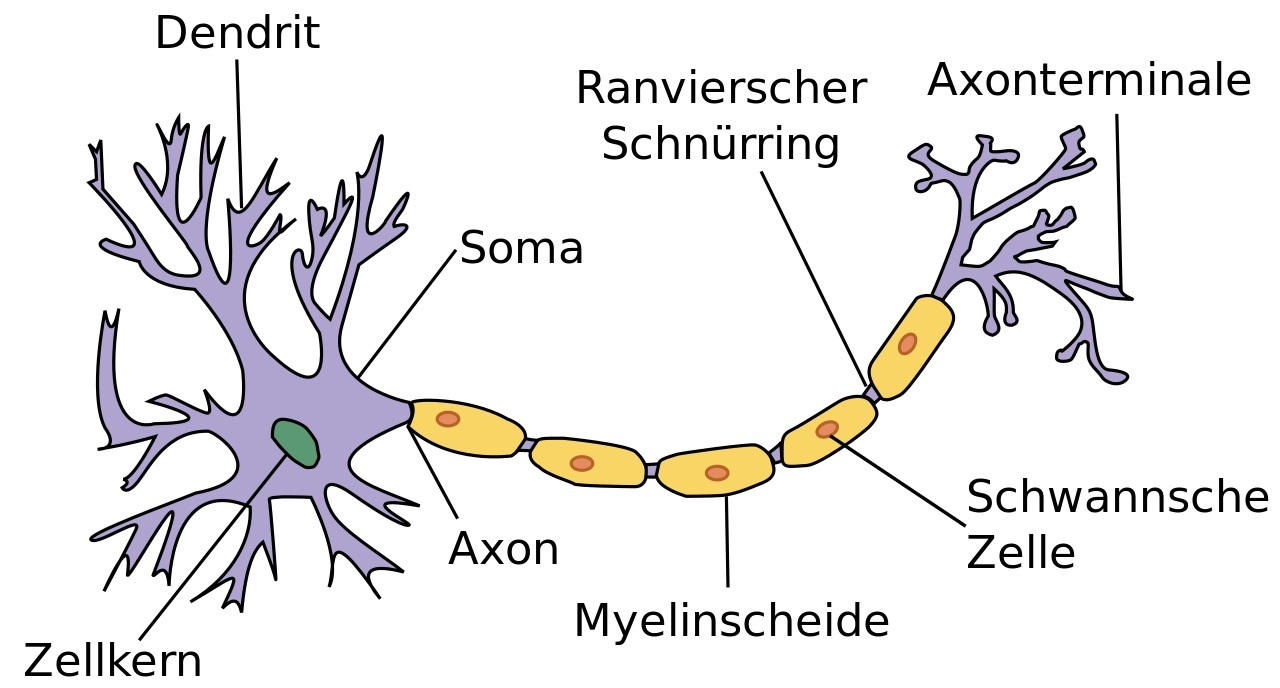
\includegraphics[width=8cm]{chapters/neural_networks/neuron.jpg}

\caption{Schematischer Aufbau eines Neurons (Quelle: Wikipedia)}
	\label{img:neuron}

\end{figure}
Dendriten sind baumartige Eingänge der Nervenzelle und dienen der Aufnahme elektrischer Reize von anderen Nervenzellen und ihrer Übertragung in den Zellkern. Aufgrund ihrer Form werden mehrere Dendriten auch als Dendritenbaum bezeichnet. Die Länge der Dendriten beeinflusst die Stärke des ausgelösten Signals: je kürze ist ein Dendrit, desto stärke ist das Signal. Diese Signale werden an den Zellkörper geleitet, wo sie sich aufsummieren.

Das Axon einer Nervenzelle kann man als „Ausgang“ des Neurons bezeichnen, weil es elektrische Signale weiterleitet, die durch Ladungsunterschiede (elektrischen Potential) zwischen der Umgebung und Zellinnerem entstehen. Wenn das aufsummierte Erregungspotenzial eine bestimmte Schwelle übersteigt, wird ein Aktionspotential fester Stärke ausgelöst, dass über das Axon und den Dendriten weitergeleitet wird.

Am Ende des Axons befinden sich die Verdickungen, die auch Synapsen genannt werden (siehe Abb. 2.2). Synapsen sind mit den Dendriten anderer Neuronen verbunden. Wobei es keine direkte physikalische Verbindung, sondern einen mit Flüssigkeit gefüllten Zwischenraum gibt. Erreicht ein über dem Schwellenwert liegendes Aktionspotential die Synapse, werden sogenannte Neurotransmitter ausgeschüttet. Diese Neurotransmitter wandern durch den synaptischen Spalt und erreichen die Rezeptoren des Dendriten. Die Neurotransmitter können an den Rezeptoren binden. Entweder führt das Anbinden der Neurotransmitter zu einer Reizweiterleitung bzw. Reizverstärkung in den Dendriten oder zu einer Hemmung des Aktionspotentials, sodass die Reizweiterleitung zum Erliegen kommt.  Die durchschnittliche Anzahl an solchen Verknüpfungen beträgt ca. 14 000 pro Neuron.

\begin{figure}[h]
\centering
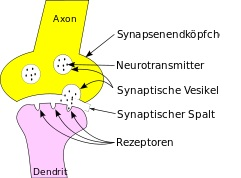
\includegraphics[width=4cm]{chapters/neural_networks/synapsen.jpg}

\caption{Synapsenkommunikation (Quelle: Wikipedia)}
	\label{img:synapsen}

\end{figure}

Der Zellkörper ist der Hauptbestandteil eines Neurons. Er ist nicht nur für die Energieproduktion verantwortlich, sondern auch für die Verarbeitung und Aufsummierung der eingehenden Signale sowie der Erzeugung bzw. Weiterleiitung der Ausgangssignale.

Die neurologischen Kenntnisse über den Aufbau menschliches Gehirns bilden die Basis für die Entwicklung mathematischer Modelle, die auch „Neuronale Netze“ genannt werden.



\section{Aufbau und Funktionsweise künstlicher  Neuronaler Netze (KNN)}


Jedes künstliche neuronale Netz hat drei Grundelemente: Neuronen, die Verbindungen zwischen den Neuronen und Lernregeln.

\subsection{Neuronen}

Ähnlich den Nervenzellen im menschlichen Gehirn sind die künstlichen „Neuronen“ die wichtigsten Bestandteile eines KNNs. Sie besitzen eine ähnliche Struktur mit vielen Ein- und Ausgängen für die Weiterleitung von ein- und ausgehenden Signalen sowie einen Körper zur Verarbeitung dieser Signale. Schematisch könnte ein künstliches Neuron folgendermaßen aussehen (siehe Abb. 3.1):

\begin{figure}[h]
\centering
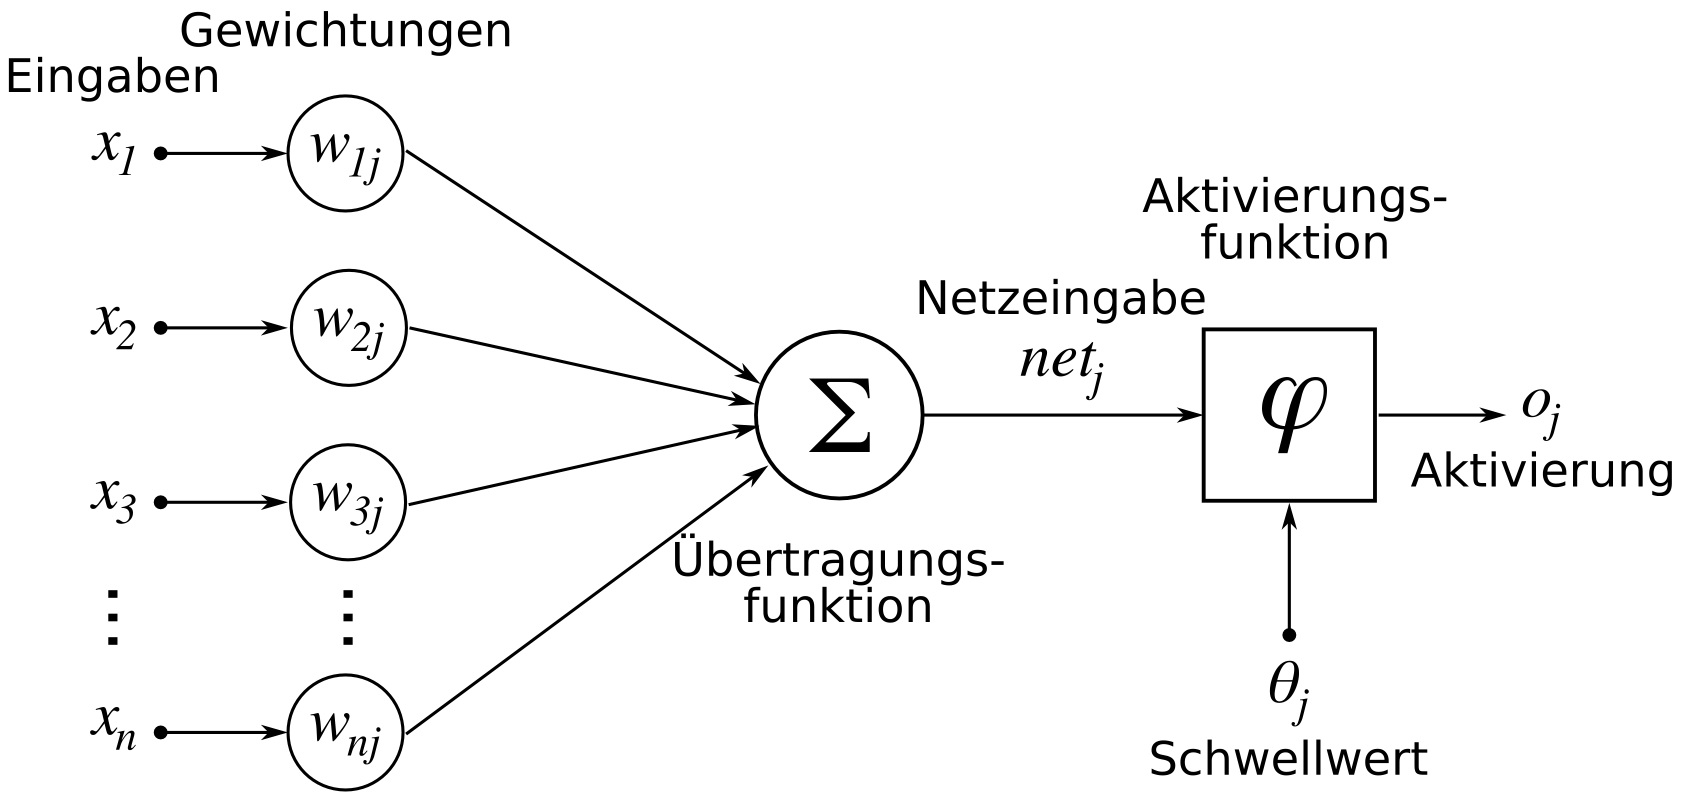
\includegraphics[width=8cm]{chapters/neural_networks/scheme.jpg}

\caption{Schematische Darstellung der wichtigsten Bestandteile eines künstlichen Neurons (Quelle: Wikipedia)}
	\label{img:scheme}

\end{figure}
Die Funktion der Dendriten erfüllen die Eingaben x$_i$, wobei i = 1, …, n. Beim modellieren eines KNN sollte man nicht vergessen, dass die Länge eines Neurons eine große Rolle bei der Bestimmung der Signalstärke spielt. Dies wird durch die Gewichtungen w$_i$$_j$ dargestellt. Die Gewichtung wird mit dem Eingabewert multiplikativ verknüpft. Es gibt verschiedene Vorgehenstechniken bei der Belegung der Gewichtungen, aber häufig werden dafür zufällige Werte in einem bestimmten Wertebereich ausgesucht. Je nachdem, ob die Gewichtung einen positiven oder einen negativen Wert hat, wirkt der Transmitter entweder verstärkend oder hemmend genau so wie bei den Menschen. Falls die Gewichtung gleich 0 ist, hat ein Neuron auf ein anderes Neuron keinen Einfluss.

Die Übertragungsfunktion könnte man sich als Erregungspotenzial vorstellen. In dieser Funktion, genauso wie die Signale im Zellkern, werden die Eingaben entsprechend ihrer Gewichtungen aufsummiert und zu einem Wert umgerechnet, damit man danach eine reellwertige Funktion darauf anwenden kann.
Der Schwellenwert $\theta$$_j$ dient als Schwellenpotenzial. Das Addieren eines Schwellwerts zur Netzeingabe verschiebt die gewichteten Eingaben.
Die Aktivierungsfunktion $\phi$ berechnet aus dem aktuellen Aktivierungszustand und der Netzeingabe den neuen Aktivierungswert. Dieser Wert wird dann weitergeleitet. Die Aktivierungsfunktion kann wie die echten Neuronen dem Alles-oder-gar-nichts- Prinzip folgen. Dabei wird bei der Überschreitung des Schwellenpotenzials wie bei menschlichen Neuronen ein festes Aktionspotential generiert. So eine Aktivierungsfunktion heißt auch Sprungfunktion (siehe Abb. 3.2).
\begin{figure}[h]
\centering
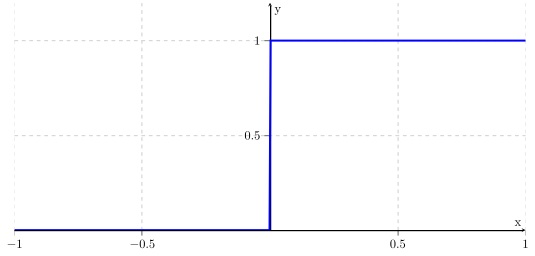
\includegraphics[width=5cm]{chapters/neural_networks/sprung.jpg}

\caption{Eine Sprungfunktion (Quelle: Wikipedia)}
	\label{img:sprung}

\end{figure}

 Eine Aktivierungsfunktion kann aber auch nach den anderen Prinzipien funktionieren. Häufig wird eine sogenannte Sigmoidfunktion (siehe Abb. 3.3) mit einer ungleichmäßigen Abhängigkeit zwischen der Ein- und Ausgabe verwendet. Weitere mögliche Aktivierungsfunktionen sind lineare oder stückweise lineare Funktionen (siehe Abb. 3.4). In solchen Funktionen hängt die Ausgabe linear von der Eingabe ab.


\begin{figure}[h]
\centering
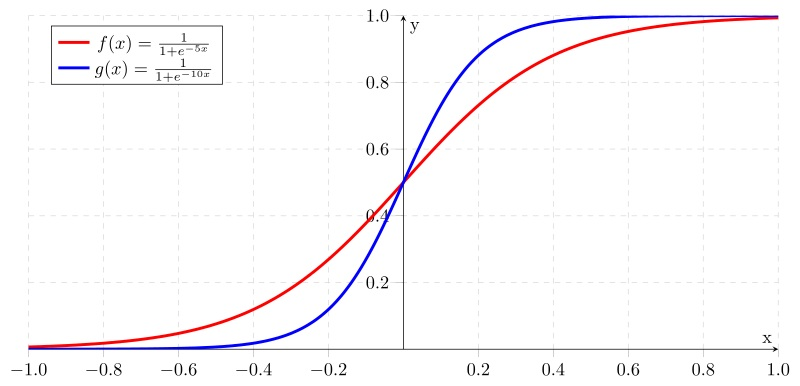
\includegraphics[width=5cm]{chapters/neural_networks/sigmoid.jpg}

\caption{eine Sigmoidfunktion mit  Steigerungsmaß (Quelle: Wikipedia)}
	\label{img:sigmoid}

\end{figure}

\begin{figure}[h]
\centering
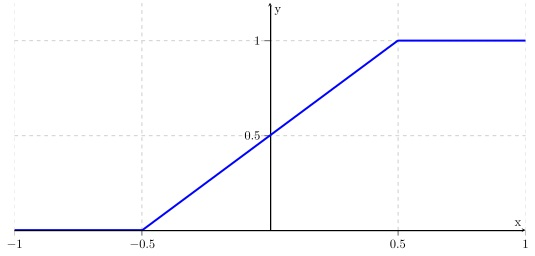
\includegraphics[width=5cm]{chapters/neural_networks/lin.jpg}

\caption{eine stückweise lineare Funktion (Quelle: Wikipedia)}
	\label{img:lin}

\end{figure}

Die Aktivierung o$_j$ ist das Ergebnis einer Aktivierungsfunktion und dient als „Ausgang“ eines künstlichen Neurons.

\subsection{Verbindungen und Netzwerktopologien}

Durch den Verbund von mehreren geordneten Kanten zwischen den Verarbeitungseinheiten entsteht ein KNN. Dabei wird die räumliche Anordnung dieser Einheiten als Netzwerktopologie bezeichnet.
Eine der wichtigsten Aufgaben der Verbindungen ist es die Architektur eines KNN festzulegen. In manchen Netzen entstehen durch solche Kanten sogenannte Schichten.

Die Verbindungen zwischen den Einheiten sind für die Kommunikation zwischen Neuronen verantwortlich: über diese Kanten werden die Daten ausgetauscht, wobei jede Verbindung durch einen Gewichtswert realisiert wird. Dabei unterscheidet man zwischen den unidirektionalen und bidirektionalen Verbindungen.

Durch unidirektionale Inter-Layer-Verbindungen werden die Daten der Eingabeschicht zur Ausgabeschicht weitergeleitet. Dadurch entstehen die sogenannten Feed-Forward-Netze, die man sich als einen azyklischen Graphen vorstellen kann.

Bidirektionale Verbindungen bilden die Feed-Backward-Netze. Bei den FB-Netzen unterscheidet man drei Typen:

a) later feedback: bidirektionale Verbindungen entstehen zwischen den Knoten einer Verarbeitungsschicht;

b) direct feedback/self-feedback: es entsteht eine unidirektionale Verbindung einer Einheit mit sich selbst;

c) indirect feedback: es entsteht eine bidirektionale Verbindung zwischen zwei Knoten aus zwei benachbarten Schichten.

Die Topologien lassen sich in drei Haupttypen unterscheiden:

a) Einschichtige Netze: solche Netze besitzen nur eine Ausgabeschicht und sind deswegen die einfachsten KNN Strukturen, die es gibt (siehe Abb. 3.5).

\begin{figure}[h]
\centering
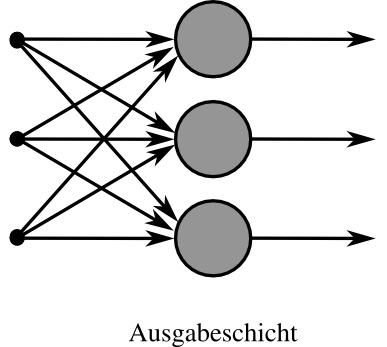
\includegraphics[width=3cm]{chapters/neural_networks/single.jpg}

\caption{Ein einschichtiges KNN (Quelle: Wikipedia)}
	\label{img:single}
\end{figure}


b) Mehrschichtige Netze: solche KNN verfügen neben der Ausgabeschicht auch über eine oder mehrere versteckte Schichten, die sich zwischen den Ein- und Ausgabeschichten befinden. Sie sind deshalb von Außen nicht sichtbar (siehe Abb. 3.6).

\begin{figure}[h]
\centering
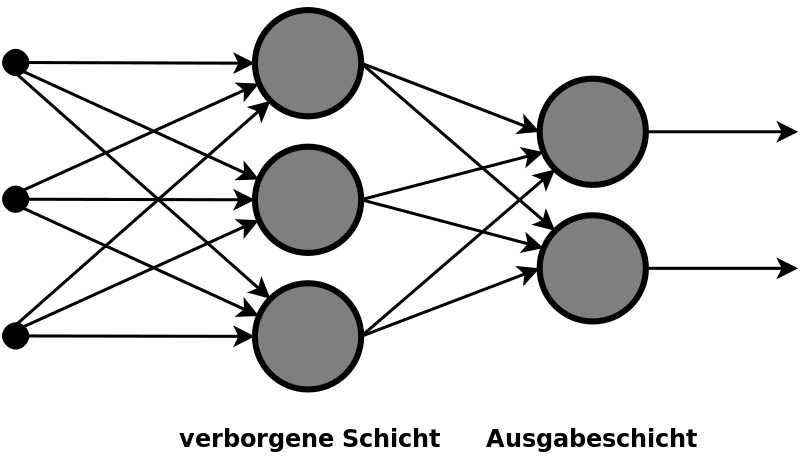
\includegraphics[width=4cm]{chapters/neural_networks/multilayer.jpg}

\caption{Ein mehrstufiges KNN mit einer verborgenen Zwischenschicht (Quelle: Wikipedia)}
	\label{img:multi}
\end{figure}

c) Rekurrente Netze: solche KNN verfügen über rückgekopellte Verbindungen, was zu Schleifen im Datenfluß führt (feedback loops). Dadurch wird der Ausgabewert eines Knotens als Eingabewert desselben Knotens verwendet (siehe Abb. 3.7).

\begin{figure}[h]
\centering
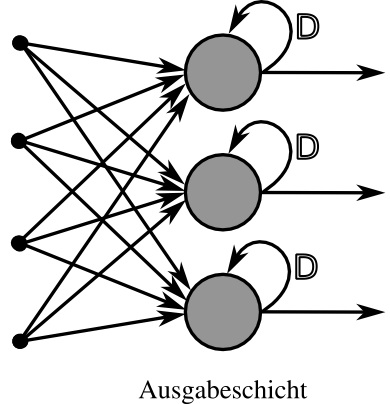
\includegraphics[width=3cm]{chapters/neural_networks/recurrent.jpg}

\caption{Ein rekurrentes KNN (Quelle: Wikipedia)}
	\label{img:recurrent}

\end{figure}

Aus diesen grundlegenden Netzwerktypen lassen sich gemischte Topologien bilden, wie z.B.: einschichtige/mehrschichtige vorwärtsbetriebene KNN (single-layer/multiple-layer feed-forward networks), Strukturen mit direkten und indirekten Rückkopplungen, Topologien mit lateralen Rückkopplungen (lateral feedback networks), u. s. w.

\subsection{Lernregeln}

Lernregeln sind eines der wichtigsten Elemente in KNN. Ihre Aufgabe ist es dafür zu sorgen, dass das Netz aus Fehlern lernt. Beim Auftreten eines Fehlers werden die Gewichte und/oder die Topologie des KNN verändert.

\subsubsection{Hebbsche Lernregel}

Diese Regel wurde im 1949 von Donald Olding Hebb aufgestellt und gilt als universelles Lernprinzip eines KNN. Diese Regel besagt, dass wenn zwei verbundene Neurone gleichzeitig aktiv sind, die Verbindung zwischen diesen Neuronen stärker ausgeprägt wird:

%\centering
$\Delta$w$_i$$_j$ = $\eta$a$_i$o$_j$ = $\eta$ $*$ g(a$_i$, t$_i$) $*$ h(o$_j$, w$_i$$_j$) ,
\newline
 wobei:  $\Delta$w$_i$$_j$ - die Veränderung des Gewichtes zweier Neuronen i und j,  $\eta$ - eine Lernrate (konstant), a$_i$ - Aktivierung von Neuron i, o$_j$ - Ausgabe von Neuron j.

Zusammen mit der Hebbschen Lernregel wird häufig eine binäre Aktivierungsfunktion benutzt. Dabei werden die Aktivierungen auf 1 oder -1 festgelegt. Das resultiert entweder in einer positiven Verstärkung oder in einer Verringerung der Gewichte, falls beide Neuronen nicht übereinstimmen.
\subsubsection{Delta-Regel}

Die Delta-Regel gilt als Weiterentwicklung der Regel von Hebb und berücksichtigt die Differenz zwischen der erwarteten Aktivierung t$_i$ (teaching output) und der tatsächlichen Aktivierung a$_i$:

$\Delta$w$_i$$_j$ = $\eta$$\delta$$_i$o$_j$ = $\eta$(t$_i$ - a$_i$)o$_j$ .

 Diese Regel wird nur zusammen mit den linearen Aktivierungsfunktionen eingesetzt.

\subsubsection{Backpropagation-Regel}

Dieses Verfahren dient zum Einlernen von KNN und ist die Verallgemeinerung von der Delta-Regel für die mehrstufigen Strukturen.
KNN versuchen die Erkennungsfehler zu minimieren, indem sie jedes Mal die Abweichung von der Lösung durch das Netz rückwärts laufen lassen. Dadurch wird das KNN so angepasst, dass die Fehler besser erkannt werden.

Die standartisierte Delta-Regel führt bei zu kleinen Abweichungen zu keiner ausreichenden Informationstiefe und ist durch die Abhängigkeit von linearen Aktivierungsfunktionen in ihrer Anwendung beschränkt. Zur Lösung dieses Problems wird die Sigmoidfunktion, die selbst kleineste Abweichungen mit nichtlinearen Aktivierungsfunktionen warhnehmen kann, zur Anpassung der Delta-Regel zu Hilfe genommen.

$\Delta$w$_i$$_j$ = $\eta$$\delta$$_i$o$_j$,
\newline
wobei
\begin{figure}[h]
\centering
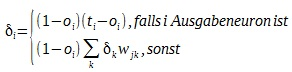
\includegraphics[width=6cm]{chapters/neural_networks/delta.jpg}

\end{figure}
\section{Beispiele}
\subsection{Das Perzeptron}
Im Jahr 1958 entwickelte Frank Rosenblatt das sogenannte Perzeptron: ein Modell, das praktisch fast alle logischen Funktionen berechnen kann. Man unterscheidet zwischen einlagigen und mehrlagigen Perzeptronen.

\subsubsection{Einlagiges Perzeptron}
\begin{figure}[h]
\centering
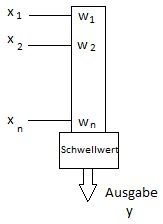
\includegraphics[width=3cm]{chapters/neural_networks/perzeptron.jpg}

\caption{Ein einlagiges Perzeptron}
	\label{img:einlagiges Perzeptron}

\end{figure}
Diese Art Perzeptronen besteht aus einer einzigen Schicht, die gleichzeitig den Ausgabevektor repräsentiert. Auf der Abbildung 4.1 ist ein einlagiges Perzeptron dargestellt. Als Eingabe bekommt es den Eingabevektor (x$_1$, ..., x$_n$).

Das Perzeptron besitzt auch einen Gewichtsvektor (w$_1$, ..., w$_n$) und einen Schwellwert $\theta$.

Aus dem Eingabe- und Gewichtsvektor berechnet man das Skalarprodukt, und wenn das Ergebnis größer oder gleich dem Schwellwert ist, dann „feuert“ unser Perzeptron.

Als Beispiel betrachten wir nun ein binäres einlagiges Perzeptron, welches eine OR-Funktion modellieren kann (siehe Abb. 4.2). Bei einer binären Eingabe besteht unser Eingabe- bzw. Gewichtsvektor nur aus zwei Werten. Die erwartete Ausgabe wird als eine Tabelle in der Abbildung 4.3 dargestellt. Unser Neuron soll nur dann „feuern“, wenn das Ergebnis 1 ist, deswegen ist es sinnvoller die beiden Gewichte auf 1 zu setzen.  Der Ausgabewert y$\in$$\{$0, 1$\}$, wobei y folgendermaßen definiert ist:
\begin{figure}[h]
\centering
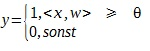
\includegraphics[width=3cm]{chapters/neural_networks/y.jpg}

\end{figure}

\begin{figure}[h]
\centering
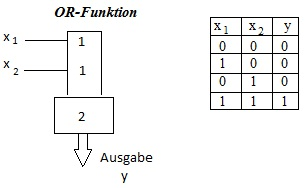
\includegraphics[width=7cm]{chapters/neural_networks/or.jpg}

\caption{Das Perzeptron-Modell einer OR-Funktionl}
	\label{img:einlagiges Perzeptron}

\end{figure}
\begin{figure}[h]
\centering
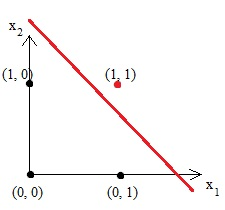
\includegraphics[width=3cm]{chapters/neural_networks/linearsep.jpg}

\caption{Linear separierbare Ergebnisse einer OR-Funktion}
	\label{img:einlagiges Perzeptron}

\end{figure}

Man sollte dabei erwähnen, dass einlagige Perzeptrone nur auf linear separierbaren Datensätzen gute Ergebnisse liefern. Linear separierbar bedeutet, dass man die Ergebnisse mit einer Linie in richtig oder falsch separieren kann. Die Abbildung 4.3 repräsentiert vier mögliche Ergebnisse aus unsem OR-Beispiel und zeigt, wie sie von einander durch eine Hyperebene separiert werden können.


\subsubsection{Mehrlagiges Perzeptron}

Mehrlagige Perzeptrone bestehen aus mindestens zwei Schichten (einer Ausgabeschicht und einer/mehreren versteckten Schicht/-en). Dabei sind alle Neuronen einer Schicht mit den Neuronen einer anderen Schicht verbunden. So eine Topologie ermöglicht die Probleme zu lösen, bei den einlagige Perzeptrone gescheitert sind.

\subsection{Perzeptron-Lernregel}

Die Lernregel eines binären einlagigen Perzeptrons könnte man folgendermaßen definieren:
\newline
w$_i$$_j$(neu) = w$_i$$_j$ (alt) $\pm$ $\Delta$w$_i$$_j$,
\newline wobei $\Delta$w$_i$$_j$ die Änderung des Gewichts w$_i$$_j$ ist. Das bedeutet:
\newline
- wenn das Ergebnis 1 und der Ausgabewert 1 sein soll, dann werden die Gewichte nicht geändert (das gleiche gilt für 0);
\newline
- wenn das Ergebnis 0 und der Ausgabewert 1 sein soll, dann werden die Gewichtungen inkrementiert;
\newline
- wenn das Ergebnis 1 und der Ausgabewert 0 sein soll, dann werden die Gewichtungen dekrementiert;

Als Beispiel betrachten wir die Funktion aus der Abbildung 4.4.

\begin{figure}[h]
\centering
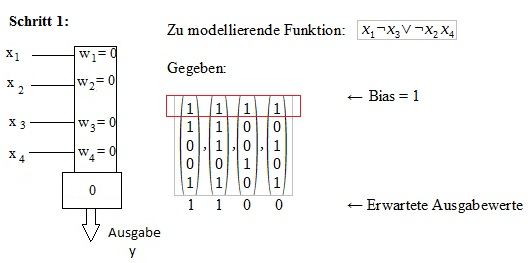
\includegraphics[width=10cm]{chapters/neural_networks/schritt1.jpg}

\caption{Eingabevektoren und Initialisierung des Gewichtsvektors}
	\label{img:einlagiges Perzeptron}

\end{figure}

Als erstes initialisieren wir den Gewichtsvektor und den Schwellenwert mit Nullen und berechnen die erwarteten Ausgabewerte. Danach berechnen wir das Skalarprodukt von den Gewichtungen und dem 1. Eingabevektor (siehe Abb. 4.5, Schritt 2). Die erwartete Ausgabe ist 1, wir bekommen aber 0 raus, deswegen müssen wir die Werte unseres Gewichtsvektors inkrementieren. Im Schritt 3 berechnen wir das Skalarprodukt von unserem neuen Gewichtsvektor und dem 2. Eingabevektor. Der Ausgabewert stimmt mit dem erwarteten Wert überein, deswegen müssen wir nichts ändern. Die gleiche Berechnung machen wir für den 3. Eingabevektor (Schritt 4) und merken, dass der Ausgabewert 0 statt 1 sein soll. Deswegen werden  die Werte des Gewichtsvektors dekrementiert. Das gleiche machen wir mit dem 4. Eingabevektor.

\begin{figure}[h]
\centering
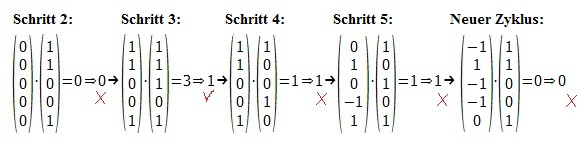
\includegraphics[width=12cm]{chapters/neural_networks/schritte.jpg}

\caption{Schritte 2-5}
	\label{img:einlagiges Perzeptron}

\end{figure}

Wenn alle Eingabevektoren getestet wurden, fängt der neue Zyklus an. Im neuen Zyklus werden die gleichen Berechnung durchgeführt, bis die passenden Gewichte gefunden sind.


\section{Fazit}

In dieser Ausarbeitung haben wir die Grundlagen und die wichtigsten Bausteine Künstlicher Neuronaler Netze kennengelernt. Zusammenfassend kann man sagen, dass KNN lernfähig sind und im Vergleich zu regelbasierten Expertensystemen keine Menschen  benötigen, die explizit beschriebene Regeln erstellen müssen. Sie sind in der Lage die Gewichtswerte und ihre Struktur an jedes Problem anzupassen und besitzen daher hohe Performanz und Adaptivitätsfähigkeit. Dank ihrer Anpassungsfähigkeit sind KNN in der Lage auch für nicht gelernte Eingaben korrekte Lösungen zu finden, deswegen hat dieses Verfahren eine Allgemeingültigkeit. KNN können nicht nur lineare, sondern auch nichtlineare Datensätze bearbeiten.

\section{Quellen und Literatur}
\begin{itemize}
\item David Kriesel. Ein kleiner Überblick über Neuronale Netze. (Online unter: \url{http://www.dkriesel.com})
\item \url{http://www2.cs.uni-paderborn.de/cs/ag-klbue/de/courses/ss03/kimas/project/downloads/AUSARBEITUNGEN/ThomasHeinenNNInMAS.pdf}
\item \url{https://de.wikipedia.org/wiki/Künstliches neuronales Netz}
\item \url{https://de.wikipedia.org/wiki/Perzeptron}
\item MIT - Lecture 12A: Neural Nets
\item MIT - Lecture 12B: Deep Neural Nets
\end{itemize}
